\section{Introduction system-environment}
\label{ch:practical_realization:sys_env}

Containerization is successfully established in Linux environments, but also available in others, like Windows and MacOS.
In Windows and MacOS, containerization via Docker is implemented through the use of an emulated Linux underneath.
Due to the recommendation to use Docker with Linux, the prototype is developed for a pure Linux environment.
The well-known and stable system Debian GNU/Linux is used as a derivative. Other Linux major distributions like the SUSE or RedHat family are not considered directly. The reason for the Debian based system is the already gained knowledge about Debian systems in the past. The compatibility to other Linux families can be easily provided by customising the path definitions. More informations about customisation and scalability is provided and demonstrated by the feature in ref bla bla.

The landscape of the system environment, including working environment is shown in Figure \ref{fig:pract:sys_env}.
\begin{figure}[h!]
 \centering
 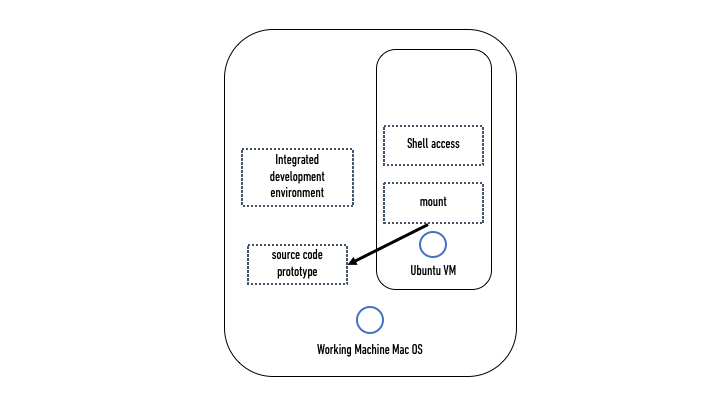
\includegraphics[width=0.6\textwidth]{gfx/examples/sys_env.png}
 \caption{System- and working environment}
 \label{fig:pract:sys_env}
\end{figure}
The working machine is a MacOS which provides locally a headless Ubuntu as a virtual machine, which is a Debian derivative. The hypervisor is the well known VirtualBox.
The code itself is written on the working machine and mounted on the virtual machine. This allows code accessing and execution on the virtual machine through a ssh tunnel. That corresponds to the idea that the prototype is operated and tested on a plain Linux system.

For this prototype Python is used as programming language. The decision of using Python can be made very straight forward in this context. First, it exists a very useful Python library for the Docker Engine API. This API allows everything the Docker command does. This means run containers, managing containers, obtaining various information and much more which is available in the official docs \cite{python_sdk}. Also, Python is an interpreted programming language. It allows it to run the same code on multiple platforms without recompilation. Hence, it is not required to recompile the code after making any alteration. This interpreting mechanism build the key features, which makes the pace of coding and testing easier and faster during the development process in the working environment. 
Furthermore, Python provides an easy syntax which is readable by any english speaker. It is like pseudocode reading, which makes it easier for non Python developers to adapt this prototype in a bigger project with another technology stack. Last but not least, Python provides a helpful module called virtual environment (venv). Virtual environments are a way to create a dedicated Python environment that allows packages to be installed, modified, and used without disturbing the global Python binary. This feature will be used to manage the necessary packages like Docker other used packages. In particular, the function is of benefit when the tool is delivered to a remote system. This tool then works independently of existing Python instances. In this context it is worth to know, that Python in version 2.x is not supported anymore since January 2020 \cite{python_deprecated}. The conclusion is that the latest version of Python is used. The same applies to the package manager Pip. The package manager should correspond to Python in a compatible version. 
Exactly versions of the this prototype is Python 3.7 and Pip3.

Now the system environment is set and which programming language has to be used as well. The next section will provide the general project structure of the prototype.